\documentclass[journal,12pt,twocolumn]{IEEEtran}

\usepackage{setspace}
\usepackage{gensymb}
\singlespacing
\usepackage[cmex10]{amsmath}

\usepackage{amsthm}

\usepackage{mathrsfs}
\usepackage{txfonts}
\usepackage{stfloats}
\usepackage{bm}
\usepackage{cite}
\usepackage{cases}
\usepackage{subfig}

\usepackage{longtable}
\usepackage{multirow}

\usepackage{enumitem}
\usepackage{mathtools}
\usepackage{steinmetz}
\usepackage{tikz}
\usepackage{circuitikz}
\usepackage{verbatim}
\usepackage{tfrupee}
\usepackage[breaklinks=true]{hyperref}
\usepackage{graphicx}
\usepackage{tkz-euclide}

\usetikzlibrary{calc,math}
\usepackage{listings}
    \usepackage{color}                                            %%
    \usepackage{array}                                            %%
    \usepackage{longtable}                                        %%
    \usepackage{calc}                                             %%
    \usepackage{multirow}                                         %%
    \usepackage{hhline}                                           %%
    \usepackage{ifthen}                                           %%
    \usepackage{lscape}     
\usepackage{multicol}
\usepackage{chngcntr}

\DeclareMathOperator*{\Res}{Res}

\renewcommand\thesection{\arabic{section}}
\renewcommand\thesubsection{\thesection.\arabic{subsection}}
\renewcommand\thesubsubsection{\thesubsection.\arabic{subsubsection}}

\renewcommand\thesectiondis{\arabic{section}}
\renewcommand\thesubsectiondis{\thesectiondis.\arabic{subsection}}
\renewcommand\thesubsubsectiondis{\thesubsectiondis.\arabic{subsubsection}}


\hyphenation{op-tical net-works semi-conduc-tor}
\def\inputGnumericTable{}                                 %%

\lstset{
%language=C,
frame=single, 
breaklines=true,
columns=fullflexible
}
\begin{document}


\newtheorem{theorem}{Theorem}[section]
\newtheorem{problem}{Problem}
\newtheorem{proposition}{Proposition}[section]
\newtheorem{lemma}{Lemma}[section]
\newtheorem{corollary}[theorem]{Corollary}
\newtheorem{example}{Example}[section]
\newtheorem{definition}[problem]{Definition}

\newcommand{\BEQA}{\begin{eqnarray}}
\newcommand{\EEQA}{\end{eqnarray}}
\newcommand{\define}{\stackrel{\triangle}{=}}
\bibliographystyle{IEEEtran}
\raggedbottom
\setlength{\parindent}{0pt}
\providecommand{\mbf}{\mathbf}
\providecommand{\pr}[1]{\ensuremath{\Pr\left(#1\right)}}
\providecommand{\qfunc}[1]{\ensuremath{Q\left(#1\right)}}
\providecommand{\sbrak}[1]{\ensuremath{{}\left[#1\right]}}
\providecommand{\lsbrak}[1]{\ensuremath{{}\left[#1\right.}}
\providecommand{\rsbrak}[1]{\ensuremath{{}\left.#1\right]}}
\providecommand{\brak}[1]{\ensuremath{\left(#1\right)}}
\providecommand{\lbrak}[1]{\ensuremath{\left(#1\right.}}
\providecommand{\rbrak}[1]{\ensuremath{\left.#1\right)}}
\providecommand{\cbrak}[1]{\ensuremath{\left\{#1\right\}}}
\providecommand{\lcbrak}[1]{\ensuremath{\left\{#1\right.}}
\providecommand{\rcbrak}[1]{\ensuremath{\left.#1\right\}}}
\theoremstyle{remark}
\newtheorem{rem}{Remark}
\newcommand{\sgn}{\mathop{\mathrm{sgn}}}
\providecommand{\res}[1]{\Res\displaylimits_{#1}} 
%\providecommand{\norm}[1]{\lVert#1\rVert}
\providecommand{\mtx}[1]{\mathbf{#1}}
\providecommand{\fourier}{\overset{\mathcal{F}}{ \rightleftharpoons}}
%\providecommand{\hilbert}{\overset{\mathcal{H}}{ \rightleftharpoons}}
\providecommand{\system}{\overset{\mathcal{H}}{ \longleftrightarrow}}
	%\newcommand{\solution}[2]{\textbf{Solution:}{#1}}
\newcommand{\solution}{\noindent \textbf{Solution: }}
\newcommand{\cosec}{\,\text{cosec}\,}
\providecommand{\dec}[2]{\ensuremath{\overset{#1}{\underset{#2}{\gtrless}}}}
\newcommand{\myvec}[1]{\ensuremath{\begin{pmatrix}#1\end{pmatrix}}}
\newcommand{\mydet}[1]{\ensuremath{\begin{vmatrix}#1\end{vmatrix}}}
\numberwithin{equation}{subsection}
\makeatletter
\@addtoreset{figure}{problem}
\makeatother
\let\StandardTheFigure\thefigure
\let\vec\mathbf
\renewcommand{\thefigure}{\theproblem}
\def\putbox#1#2#3{\makebox[0in][l]{\makebox[#1][l]{}\raisebox{\baselineskip}[0in][0in]{\raisebox{#2}[0in][0in]{#3}}}}
     \def\rightbox#1{\makebox[0in][r]{#1}}
     \def\centbox#1{\makebox[0in]{#1}}
     \def\topbox#1{\raisebox{-\baselineskip}[0in][0in]{#1}}
     \def\midbox#1{\raisebox{-0.5\baselineskip}[0in][0in]{#1}}
\pagenumbering{gobble}
\title{Assignment-2}
\author{Adil Salfi  - CS20BTECH11031}
\maketitle
Download all python codes from
\begin{lstlisting}
https://github.com/AdilSalfi/AI1103/tree/main/Assignment-2/Codes
\end{lstlisting}
and latex-tikz code from
\begin{lstlisting}
https://github.com/AdilSalfi/AI1103/tree/main/Assignment-2
\end{lstlisting}
\section*{\textbf{Problem}}
GATE-EC Question 59 : \\
Let X be a random variable having the distribution function :
\begin{align*}
F(x)=   
\begin{cases}
0 & x<0 \\
\frac{1}{4} & 0\le x<1 \\
\frac{1}{3} & 1\le x<2 \\
\frac{1}{2} & 2\le x<\frac{11}{3} \\
1 & x\ge\frac{11}{3}
\end{cases}
\end{align*}
Then $E(X)$ is equal to :

\section*{\textbf{Solution}}
\textrightarrow As the Cumulative Distribution Function $F(x)$ is discontinuos and is similar to a step function, it represents the CDF of a discrete Random Variable.\\[1mm]
\textrightarrow As the CDF is discontinuos when $x=(0,1,2,\frac{11}{3})$, Random Variable $X \in \{0, 1, 2, \frac{11}{3}\}$. \\[1mm]
\textrightarrow The probabilites for each value of $X$ are calculated below using the formula: 
\begin{align*}
\pr{X=i}=F(b)-F(a),\hspace{4pt} i \in [a,b] \tag{1} \label{1}
\end{align*}

1) Calculation of \pr{X=0}: \\[2mm]
Using \eqref{1},
\begin{flalign*}
\rightarrow &\pr{X=0}=F(0.5)-F(-0.5)=\frac{1}{4}-0& \\
\therefore &\pr{X=0}=\frac{1}{4}& \tag{2} \label{2} 
\end{flalign*}
\newpage
2) Calculation of \pr{X=1}: \\[2mm]
Using \eqref{1},
\begin{flalign*}
\rightarrow &\pr{X=1}=F(1.5)-F(-0.5)=\frac{1}{3}-\frac{1}{4}& \\
\therefore &\pr{X=1}=\frac{1}{12}& \tag{3} \label{3} 
\end{flalign*}

3) Calculation of \pr{X=2}: \\[2mm]
Using \eqref{1},
\begin{flalign*}
\rightarrow &\pr{X=2}=F(2.5)-F(1.5)=\frac{1}{2}-\frac{1}{3}& \\
\therefore &\pr{X=2}=\frac{1}{6}& \tag{4} \label{4} 
\end{flalign*}

4) Calculation of \pr{X=\frac{11}{3}}: \\[2mm]
Using \eqref{1},
\begin{flalign*}
\rightarrow &\pr{X=\frac{11}{3}}=F(4)-F(3)=1-\frac{1}{2}& \\
\therefore &\pr{X=\frac{11}{3}}=\frac{1}{2}& \tag{5} \label{5} 
\end{flalign*}
\\
\textbf{For Discrete Random Variables}
\begin{align*}
E(X)&=\sum_{i=1}^{n} x\pr{x} \tag{6} \label{6}
\end{align*}
Using \eqref{2},\eqref{3},\eqref{4} and \eqref{5}
\begin{align*}
\begin{split}
    &=(0\times \frac{1}{4})+(1\times \frac{1}{12})+(2\times \frac{1}{6})+(\frac{11}{3}\times \frac{1}{2}) \\
    &=\frac{27}{12} \\
    &=2.25 \\
\end{split}
\end{align*}
\begin{align*}
\therefore E(X)=2.25 \tag{7} \label{7}
\end{align*}
\newpage
\begin{figure}[ht]
    \centering
    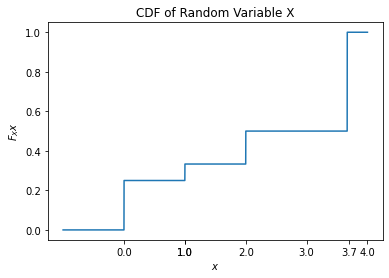
\includegraphics[width=\columnwidth]{CDF.png}
    \caption{CDF of X}
    \label{fig:1}
\end{figure}
\vfill\eject
\begin{figure}[ht]
    \centering
    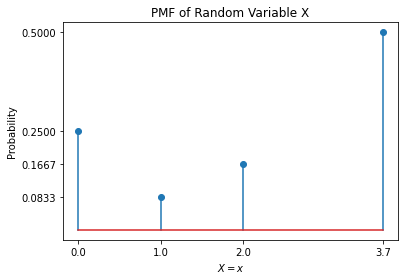
\includegraphics[width=\columnwidth]{PMF.png}
    \caption{PMF of X}
    \label{fig:2}
\end{figure}
\end{document}
